\chapter{Metastability and phononic CDW quench in TaTe2}

Ever since the proposition of Graphene as a model system for more complex materials, researchers were extremely successful in finding new physical properties of Graphene itself and extending the knowledge to other materials.
This resulted in the explosion of the field and discovery of many new phenomena, from xyz to superconductivty in magic angle twisted bilayer graphene.
These developments ultimately also resulted in the wish for the emergence other platforms, that could drive new ideas and discoveries.
One of these platforms of 2D materials are transition metal dichalcogenides (TMDs).

introduce some more the other tmds and developments here, especially for ultrafast

One constituent of these TMDs is \ce{TaTe2} which, compared to its \ce{TaX2} based sister compounds \ce{TaS2} and \ce{TaSe2} and the isostructural polytypes of \ce{MTe2} like \ce{NbTe2} or \ce{VTe2}, it has so far received less attention from the community, but many reports characterizing the compound have come up in recent years, as well as the first ultrafast out-of-equilibrium studies.
\ce{TaTe2} can be characterized as semimetal at room temperature (RT) and forms ribbon like structures in a distorted 1T'-phase.
The compound appears to have strong molecular properties, with \ce{Ta} atoms forming in trimers or fluctuating dimers, with each \ce{Ta}-atoms being surrounded by 8 \ce{Te}-atoms.
At \SI{170}{\kelvin} the material undergoes a structural phase transitions, where two \ce{Ta}-atoms further distort the structure, breaking dimers and instead form "butterfly" shaped heptameres in a 1T"-phase.
This structural phase transition is accompanied by the formation of charge density wave (CDW), which has been observed both by gap formation in ARPES and the formation of a periodic lattice distortion (PLD) in STM and diffraction.
The exact mechanism of how this phase transition occurs and what the interplay with the CDW is have still not been understood.

\begin{figure}
	\centering
	\subfigure[]{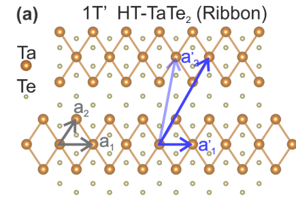
\includegraphics[width=0.33\textwidth]{tate2/ht_structure.png}}
	\subfigure[]{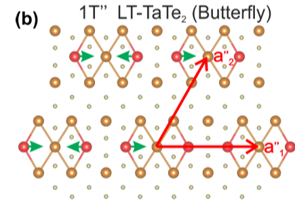
\includegraphics[width=0.33\textwidth]{tate2/lt_structure.png}}
	\subfigure[]{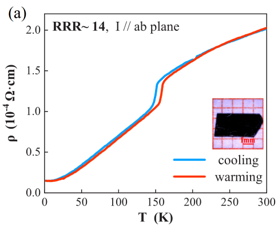
\includegraphics[width=0.33\textwidth]{tate2/resistivity.png}}
	\caption{(a) 1T' RT phase of \ce{TaTe2} forming ribbons. (b) 1T" LT phase of \ce{TaTe2}, \ce{Ta} atoms move together forming heptameres. (c) Resistivity of \ce{TaTe2} as a function of temperature with an overall reduction in resistivity while cooling. A phase transition occurs at \SI{170}{\kelvin}, which is accompanied by a further steplike reduction in resistivity.}
	\label{fig:tate_structure}
\end{figure}


The reason for the lack of understanding stems from the electronic reaction to the phase transition, especially in comparison to the \ce{TaX2} sister compounds.
Typically, entering a CDW phase by cooling the sample down from RT leads to an increase in resistivity due to the reduced density of states (DOS) in proximity to the Fermi level $E_F$.
Similarly a drop of the magnetic susceptibility would be expected while cooling $T_s$.
Instead \ce{TaTe2} shows a drop in resistivity and an increase in magnetic susceptibility, despite the observation of small gaps in the band structure.
For this reason the compound has been branded a "strange" CDW material.

In this chapter of the thesis I give further insight into the driving mechanism of the CDW and the formation of the structural phase transition with the help of ultrafast pump-probe ARPES, and comparing our data to the recent ARPES and ultrafast publications on \ce{TaTe2}.
Our data shows strong oscillations, a delayed quench of the CDW gap after laser excitation and a metastable state at high fluences persisting for $>\SI{100}{\pico\second}$.

\section{Bandstructure and Fermiology}


\section{Ultrafast charge dynamics and CDW quench}


\section{Energy and momentum resolved electron-phonon coupling}


\section{Metastability}


\section{Conclusion and Outlook}
